%sf bay is screwed
We focus on the San Francisco Bay Area, a seismically-active region with a complex web of roads and transit networks, to illustrate our approach (Figure~\ref{fig:equity_study_area}). The area follows a polycentric metropolitan form, with San Francisco as the primary center and other jobs  concentrated in suburban centers, such as Silicon Valley~\cite{cervero_polycentrism_1997}. The region has a wide array of trip patterns for mandatory and non-mandatory trips. Furthermore, trip times and routes vary greatly depending on travel preferences and workplace locations~\cite{cervero_polycentrism_1997}. Thus,  we might expect noticeable disparities between households in the risk of travel time delays due to earthquakes. 


%and here are the study area and models
We consider the road network and the relevant transit systems. We  model damage to bridges and other structures from a probabilistic set of earthquake events in order to predict the loss in mode-destination accessibility. This performance measure is popular in urban planning~\cite[e.g.,][]{geurs_accessibility_2004,kockelman_travel_1997,waddell_incorporating_2002}. Mode-destination accessibility, hereafter referred to as accessibility, measures the distribution of travel destination opportunities weighted by the composite utility of all modes of travel to those destinations, i.e., the ease of someone getting to different destinations weighted by how desirable those destinations are~\cite{handy_measuring_1997,niemeier_accessibility:_1997}. The utility function for the mode-destination choice may be estimated using a multinomial random utility model where the logsum represents the accessibility value~\cite{manski_structural_1981,handy_measuring_1997,niemeier_accessibility:_1997}. Namely, accessibility for a particular agent $a$ is
\begin{equation}
Acc_a = \ln \left[ \sum_{\forall \in C_a} \exp (V_{a(c)}) \right],
\label{eq:acc}
\end{equation}
where $V_{a(c)}$ is the utility of the $c^{th}$ choice for the $a^{th}$ person for $a = 1, \ldots, A$, and $C_a$ is the choice set for the $a^{th}$ person~\cite{handy_measuring_1997}. Choices refer to travel destinations and the mode of travel (driving, walking, bus, etc.). The units are a dimensionless quantity, $utils$. As an extension, the accessibility values from the previous equation can be converted into equivalent time and dollar amounts using \emph{compensating variation} for cost-benefit studies; for the case study, 0.0134 $utils$ (generic measure of utility) equals the value of one minute per day~\cite{niemeier_accessibility:_1997,small_applied_1981,ory_personal_2013} and we conservatively value one hour of time as approximately \$15~\cite{united_states_department_of_transportation_revised_2011}. In other words, one $util$ is worth approximately \$20 per person per day based on these assumptions. With nearly 7 million people in the region, even small changes in $utils$ lead to large economic losses. Since accessibility measures how easily people can get to the destinations they desire, accessibility is used as one of the measures of human welfare~\cite[e.g.,][]{niemeier_accessibility:_1997}.

%no surprises
From a large set of ground-motion intensity maps and damage maps, we choose a set of forty maps, using the optimization procedure we proposed in Miller and Baker~\cite{miller_ground-motion_2014}; we chose the fixed-demand travel time delay as the proxy metric, because it is related to travel time delays expected in the high-fidelity model. We then use the high-fidelity model to predict the transportation network impacts of the forty pairs of ground-motion intensity and damage maps. Readers are referred to Miller~\cite{miller_seismic_2014} for a step-by-step procedure for aggregating the requisite data sources, modeling interdependencies, and adapting an activity-based transportation model for catastrophe risk assessment. The outcome is forty sets of results for the target performance metric, mode-destination accessibility. Each accessibility value has a corresponding annual rate of occurrence.
In the following sections, we first compare region-wide results, and then focus on particular characteristics of three communities (Figure~\ref{fig:equity_study_area} shows the study area and three communities). Finally, we discuss generalizable trends.
\begin{figure}
\centering
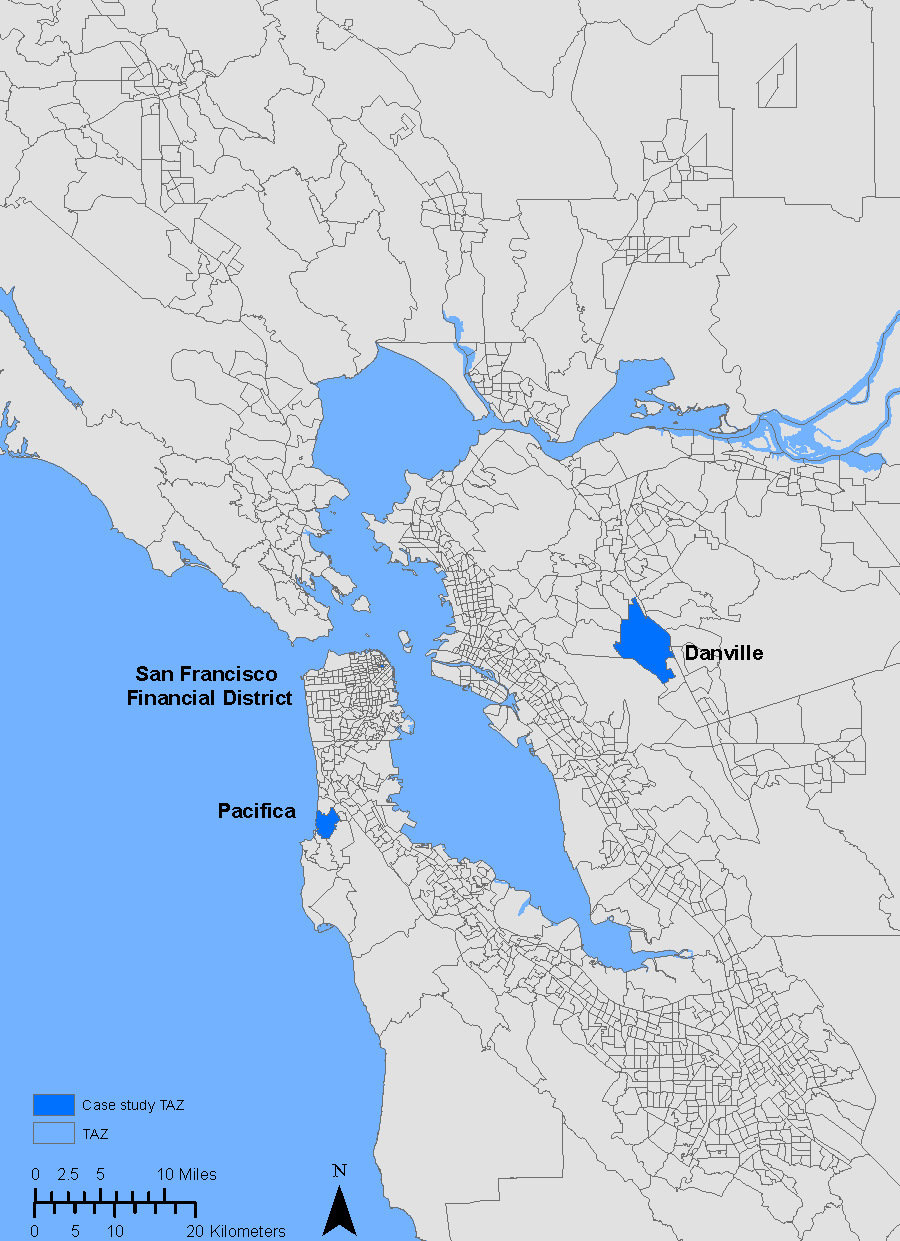
\includegraphics[width=6in]{FIGS/equity_case.pdf} 
\caption{Study area: San Francisco Bay Area, CA with specific travel analysis zones (TAZs) used in the case study marked in blue.}
\label{fig:equity_study_area}
\end{figure}

